\chapter{Current APIs\label{section:currentAPIs}}
\section{Argus}
%https://docs.nvidia.com/jetson/l4t-multimedia/group__LibargusAPI.html

Argus is a camera API that is developed by Nvidia. Argus runs only on Nvidia
hardware, such as the Jetson Orin Nano Developer Kit.

Argus is roughly based on V4L2 though effectively a re-implementation. At the
time Argus was created, V4L2 was still in an early stage. It di not supporting
a variety of features such as multicamera setups etc. hence Argus was created
in order to add the missing features easily. These days V4L2 and Argus are very
close though in later chapters we will give an overview of what pros and cons
each has.

The reason Argus does not use V4L2 is largely a historical one at this point.
At the time Argus was created V4L2 was in an early stage, it had very limited
features. Nvidia created Argus in order to leviate these issues but ended up
with an API that is very similar to V4L2. Automotive for example needed support
for multi camera use cases, this was something that was not supported in V4L2 at
the time.

Over time, the API has aged a little though. Today it is still very dependent on
EGL. EGL is a very dated API, like OpenGL it is largely in maintenance mode
today.

\section{libcamera}
libcamera is an open-source C++ embedded camera framework that supports a large
number of complex cameras such as the Sony IMX 219, 477 and many more. It
supports multiple encoders to receive images in for example PNGs/raw images.
The primary target for libcamera is Arm processors in the form of Raspberry
PI's, Chrome OS and Android though many other architectures are also supported
\cite{libcameraStack}. Because image processing algorithms are often
proprietary and very secret, libcamera also allows for binary blobs to be
supplied by the vendors. The vendors do need to submit the "base case" where
the camera can take a still image with decent quality to get the blob approved.

\begin{figure}
    \begin{center}
        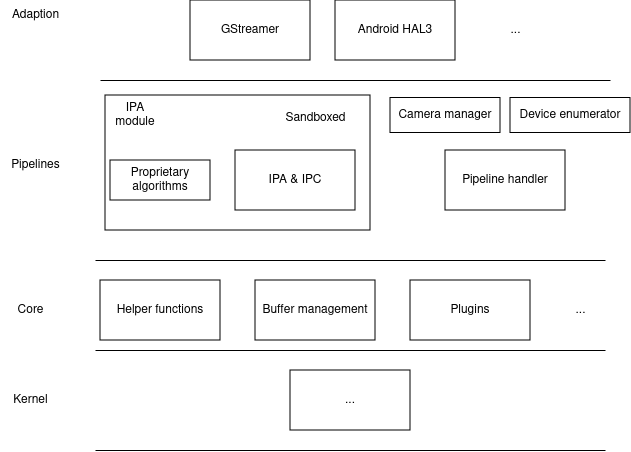
\includegraphics[width=0.60\textwidth]{figures/libcameraarch.png}
    \end{center}
    \caption{High level overview of how the libcamera architecture looks like}
    \label{fig:libcameraarch}
\end{figure}


\section{HAL3}
Hardware Abstraction Layer 3 (HAL3) is the camera API that is included in each
Android phone, it has remarkable features for a mobile phone camera. It was
created to bridge the gap between the higher level the API camera2 and the
lower level hardware APIs. It allows for more modification than camera2, while
requiring more work to manage.

Like libcamera and Argus, it is a request based API. Being a request based API
allows it to be a very explicit API and allows for the user to have a
significantly higher level of control. The reason for the other
two being very close to HAL3 in style is because they are largely based on it.
Argus does not provide an interface for this but the style is similar. libcamera
does provide an interface for it.

While request based APIs allow for a better control of the camera, it also
makes it so that the API is not able to optimze much if the request can fully
change each frame. While if the API was a streaming API it could have certain
assumptions that reduce amount of copies. Hence making it faster.

In \cref{fig:hal3arch} we can see the high level diagram of how a capture
request is done and how the frame arrives to the end user. The capture process
works in the following way:

\begin{enumerate}
    \item Create a capture request, modifying gain, focal length etc.
    \item Give capture request to the capture device class
    \item Capture device passes the request to the ISP which creates a program
        for the request, see \cref{section:isp} for a detailed explanation of
        how ISPs work.

    \item Images come in the form of a capture result to the application.
\end{enumerate}


\begin{figure}
    \begin{center}
        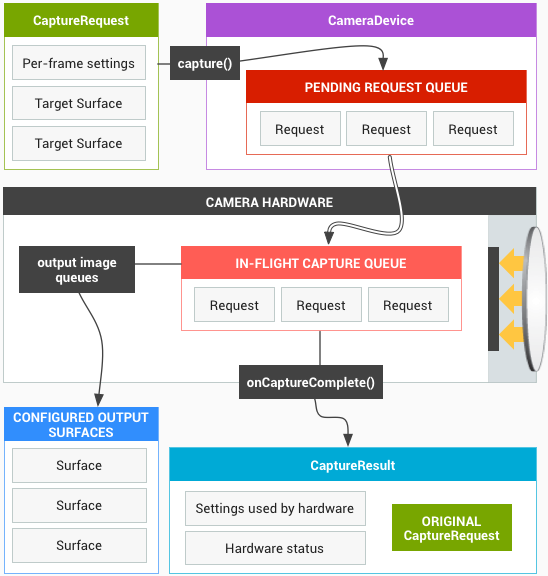
\includegraphics[width=0.5\textwidth]{figures/hal3arch}
    \end{center}
    \caption{HAL3 architecture \cite{hal3arch}}\label{fig:hal3arch}
\end{figure}

\section{Kamaros}
Over the years there have been some camera standardization efforts such as
OpenKCam. These have failed though due to lack of industry interest. Today
the Khronos group has started the camera standardization effort again with
Kamaros.

Kamaros is a new API currently (2024) being designed. Its goal is to
standardize embedded camera frameworks. This means that instead of needing
three different APIs for Android, L4T, and Linux you would only need to use
Kamaros. It would sit on top of the transport layer (CSI-2, USB etc.), allowing
the applications to use a single API to communicate with cameras over multiple
platforms. Though there are still many issues in the camera world that will not
be solved by Kamaros. Examples of these are for example camera configuration.
Currently there is no standard way to configure cameras, the camera drivers are
often a huge part of the code base. At the same time, there is not a lot of
difference between them. In the future, Kamaros may try to tackle this problem
though it is not anything that will be solved initially.

The API is under development, so not much can be mentioned about the API itself
due to a spec not being out yet. It hopes to be easy to use and ability to
leverage Vulkan for post processing. This would allow users to easily create
cross platform code and not be highly platform dependent as it is currently.
\cref{fig:kamaros_stack} shows where it would fit in a typical application.

\begin{figure}
    \begin{center}
        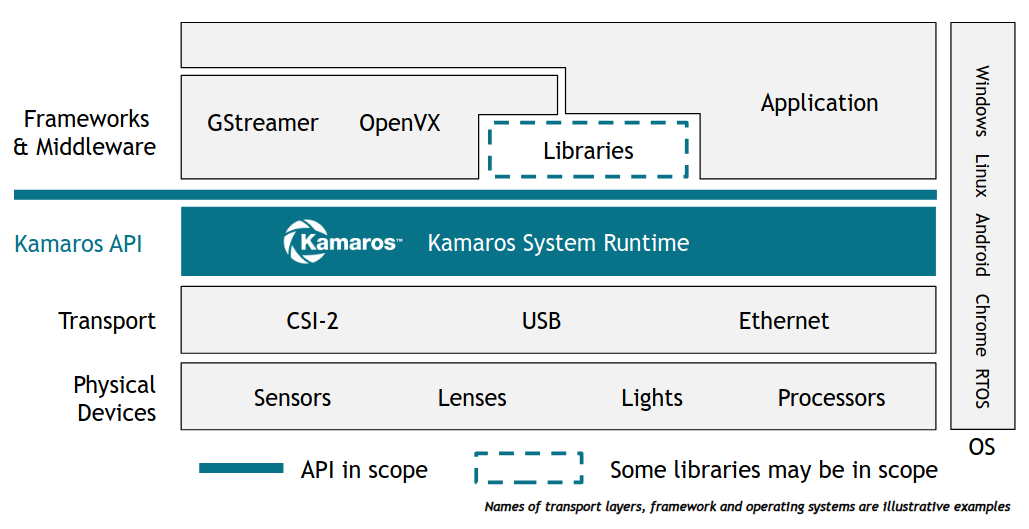
\includegraphics[width=0.60\textwidth]{figures/kamaros_stack.png}
    \end{center}
    \caption[Kamaros stack]{Kamaros stack\footnotemark}\label{fig:kamaros_stack}
\end{figure}
\footnotetext{https://www.khronos.org/assets/uploads/developers/presentations/Khronos\_Kamaros\_Embedded\_World\_Mar23.pdf}

\section {GenICam}
\textit{Generic Interface for Cameras} (GenICam) is a standard that was
developed by the \textit{European Machine Vision Association} (EMVA). It is
largely used by industry.

Genicam is a significantly higher level API than the ones listed above. It
uses for example XML files to configure cameras, this is not very space
efficient compared to device trees. In general it is not really built for
embedded use cases.

% TODO?

